
\chapter{Requirements Analyse} % Chapter title

\label{requirementsAnalyse} % For referencing the chapter elsewhere, use \autoref{ch:InOnderzoek}
Om inzicht te krijgen in de eisen van de nieuwe module naast de eisen die al vermeld staan in de opdracht. is er een intake gesprek geweest met de CTO (Bas Breier), in dit gesprek is aan bod gekomen wie de stakeholders zijn en welke requirements hij heeft naast de requirements die in de opdracht staan. In dit gesprek is er meer ingegaan op de details van het functioneren van de module. Ook is er een beeld geschets over de huidige situatie en naar welke situatie er gegaan moet worden. % nog ff aanpassenin ABN Het verslag is
Zie in Appendix A.XX het verslag van dit interview.


\section{Huidige situatie}
In de huidige situatie wordt er een SOUP analyse gedaan door de ontwikkelaars op het moment dat een project ontwikkeld wordt. dit is veelal handmatig zoeken in online resources op bibliotheken die gebruikt worden. Dit neemt veel kostbare tijd in beslag die beter besteed kan worden om nieuwe features toe te voegen. Daarnaast worden de bevindingen die gedaan worden niet centraal opgeslagen zodat er een potentie is dat niet iedereen op de hoogte is van de actuele informatie.

\section{Gewenste situatie}
De gewenste situatie is dat projectmanagers, ontwikkelaars en het dagelijks bestuur real-time inzage hebben in de huidige staat van de kwetsbaarheden in de gebruikte externe bibliotheken. Dit is te doen door een onderdeel in een portal te bouwen die op een overzichtelijke manier deze informatie weergeeft.

om de informatie weer te kunnen geven moet er een manier worden gevonden om tijdens een bouwprocess de versies van de gebruikte bibliotheken te achterhalen. En deze vervolgens tegen een Vulnerability Database te leggen. Deze gegevens dienen in een interne database opgeslagen te worden waarop de het onderdeel in de portal gegevens op kan halen. Waarop vervolgens door de stakeholders de gewenste informatie gehaald kan worden.

\section{De stakeholders}
De stakeholders kunnen opgedeelt worden in twee hoofdgroepen(Tabel 1): externe en interne stakeholders. De klant is als enige een externe stakeholder en is buiten de analyse gehouden omdat deze staceholder alleen indirect resultaten bemerkt doormiddel van het verkrijgen van verbeterde software. De klant als stakeholder is dus passief en zal niet worden geinterviewt. Met personen uit de interne stakeholders groepen zijn interviews gehouden om een inzicht te krijgen in hun belang en invloed bij de module. Daarnaast is er een eerste lijst met requirements opgesteld waaraan de module dient te voldoen. Deze lijst is een start en zal na enkele sprintdemo's worden aangepast of uitgebreid. Na iedere tweede sprint zal een evaluatie worden gehouden om inzicht te krijgen of de requirements nog accuraat zijn en eventueel nog moeten worden aangescherpt.
De belangen en invloeden worden in de komende subsecties verder toegelicht.

\subsection{Dagelijks bestuur (intern)}
Het dagelijks bestuur ziet vooral voordelen in het inzicht krijgen van kwetsbaarheden op een overzichtelijke manier, zodat ze kunnen sturen in het gebruik van biblioteken of andere technologi\"en. Echter zien zij ook kosten gemoeid met de verandering. Door de manier van werken dienen deze kosten terug verdient te worden door werkzaamheden binnen andere projecten. De CTO ziet vooral tijdswinst zodat de time-to-market voor andere projecten hoger ligt en dus meer verdient kan worden.
\subsection{Projectmanagers (intern)}
Project managers krijgen op dit moment een update over de staat van kwetsbaarheden tijdens stand-ups en aan het einde van een sprint tijdens de sprint demo's. De nieuwe module biedt ze de mogelijkheid om up-to-date informatie on-demand te verkrijgen. Op de vraag of het het waard is dat een aantal ontwikkelaars tijd kwijt zijn in testen en meedenken over de module weegt volgens hen op tegen de voordelen die de module in de toekomst kan brengen.
\subsection{Ontwikkelteam (intern)}
Het ontwikkelteam wil graag meedenken en meewerken aan een oplossing, gezien zij de gene waren die handmatig de analyse uitvoerden. Zij zien voor een oplossing voor een taak dat veel tijd in beslag nam en afleide van de daadwerkelijke taak.
\subsection{Klant (extern)}
Als laatste de klant welke een passieve stakeholder is gezien zij niet direct betrokken zijn bij de ontwikkeling van de module maar wel verbeteringen genieten in de zin van veilige en betrouwbare software.

%tabel nog in vorm brengen eerste kolom is veel te breed.
\begin{table}[H]
%\myfloatalign
  \begin{tabularx}{\textwidth}{Xll}
  \toprule
  \tableheadline{Groep}   & \tableheadline{Stakeholder}\\
  \midrule
  Extern                  & Klant                      \\
  \midrule
  Intern                  & Dagelijks Bestuur          \\
                        & Project managers           \\
                        & CTO                        \\
                        & Ontwikkelaars              \\
  \bottomrule
  \end{tabularx}
  \caption[Verdeling stakeholders]{Verdeling stakeholders}
  \label{tab:verdeling_StakeHolders}
\end{table}
\subsection{Stakeholder analyse}
\begin{figure}[H]
\myfloatalign
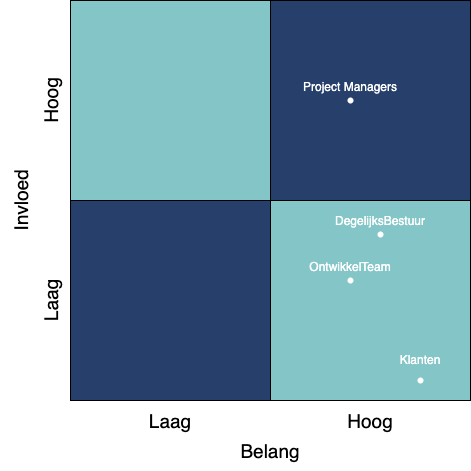
\includegraphics[width=10cm]{gfx/stakeholderanalyse}
\caption{StakeHolders Analyse}
\label{fig:StakeholderAnalyse}
\end{figure}
Zoals te zien is in figuur[X] zijn de projectmanager, het ontwikkelteam en de klanten het meest gebaad bij een nieuwe module voor de analyse van kwetsbaarheden. Echter zijn de klanten niet tot bijna niet betrokken bij de ontwikkeling van de module maar hebben er indirect wel belang bij omdat de software die voor hen ontwikkeld wordt veiliger wordt door het voeren van een geautomatiseerde analyse. Door deze analyse worden alleen de requirements meegnomen die intern zijn opgenomen.
\section{Requirements}
Naast het analyseren van de betrokkenheid en belang van de stakeholders is er ook gevraagd welke requirements ze terug wilden zien in de applicatie en welke prioriteit er aan gesteld werdt. Om een leidraad te verschaffen is de MoSCoW-methode gebruikt. Hieronder is een lijst geformuleert met de belangrijkset requirements vanuit de stakeholders. Deze lijst is niet volledig en wordt na iedere sprint aangepast aan de resultaten van de sprint ervoor.\\

\textbf{Must Have Moet nog onderverdeeld worden in MoSCoW}
\begin{itemize}
  \item Als \textit{gebruiker} wil ik dat de SOUP module in de portal te vinden is zodat alle tools die gebruikt worden binnen Eaglescience op een enkele plek te vinden zijn.
  \item Als \textit{gebruiker} wil ik een overzicht per project kunnen zien met daarin de gebruikte bibliotheken zodat ik inzage heb ik wat er gebruikt wordt voor ontwikkeling.
  \item Als \textit{gebruiker} wil ik een overzicht per project zien welke kwetsbaarheden er zich in bibliotheken bevinden, zodat ik actie kan ondernemen om de software nog veiliger te maken.
  \item Als \textit{gebruiker} wil ik in kunnen loggen met mijn LDAP? account zodat ik niet nog een keer een username/wachtwoord combinatie hoe te leren.
  \item Als \textit{gebruiker} wil ik een project kunnen toevoegen zodat ik ook van dat project de kwetsbaarheden in kan zien en deze software ook veilger wordt.
  \item Als \textit{Module} wil ik een update krijgen van de laatste build met specifiek de laatste kwetsbaarheden, zodat ik deze kan weergeven in de portal.
  \item als \textit{module} wil ik
  \item Als \textit{gebruiker} wil ik dat periodiek automatisch een check analyse wordt uitgevoerd zodat ik er zelf niet naar om hoef te kijken.
  \item Als \textit{gebruiker} wil ik zelf een analyse kunnen starten voor een project zodat ik een up-to-date versie heb van de resultaten.
  \item Als \textit{Project manager} wil ik projecten kunnen toevoegen aan de module, zodat ook deze mee genomen worden in de automatische analyse.
  \item Als \textit{Project manager} wil ik ontwikkelaars kunnen toevoegen aan een project zodat deze ook inzicht krijgen in de huidige stand van zaken.
  \item Als \textit{Project manager} wil ik een notificatie( via mail/rocketchat) ontvangen als er een
\end{itemize}

\textbf{Should Have}
\begin{itemize}
  \item Moeten nog voorkomen uit de prioriteit analyse
\end{itemize}

\textbf{Could Have}
\begin{itemize}
\item
\end{itemize}

\textbf{Won't Have}
\begin{itemize}
  \item Moeten nog voorkomen uit de prioriteit analyse
\end{itemize}
De Won't haves staan hierbij genoemd als leidraad voor eventueel updates in de toekomst. Als blijkt dat er tussen de won'ts toch low hanging fruit blijkt te hangen kunnen deze meegenomen worden in de sprints. De requirements worden als epics in een JIRA omgeving gezet om vervolgens een planning te kunnen maken.


\section{WerkWijze en planning}
Binnen Eaglescience wordt er scrum gewerkt en ook al ben ik als enig werkzaam op dit project zal er zoveel mogelijk op deze manier worden gewerkt inhoudend dat een sprint 2 weken duurt met aan het begin een springplanning en aan het einde van de sprint een demo en een retrospective zal worden gehouden. De daily stand-ups zal worden gehouden met de Product-owner en de reviewers van de code om zo een kortere feedback loop te krijgen. Daarnaast staan er verschillende collega's die support kunnen leveren.
